\documentclass{scrartcl}

\usepackage{amssymb}
\usepackage{amsmath}
\usepackage{tikz}
\usetikzlibrary{calc}	%for centerarc

\def\centerarc[#1](#2)(#3:#4:#5)% Syntax: [draw options] (center) (initial angle:final angle:radius)
{ \draw[#1] ($(#2)+({#5*cos(#3)},{#5*sin(#3)})$) arc (#3:#4:#5); }

\begin{document}
	
	%from Bergson - Matter and Memory, p. 128 (fig. 1)
	%NB: in some versions, the bottom part is dashed
	\begin{tikzpicture}
	\centerarc[very thick](0,-0.05)(0:180:1.54)		\node at (0,1.2) {A};
	\centerarc[very thick](0,0.7)(-25:205:1.7)		\node at (0,2.1) {B};
	\centerarc[very thick](0,1.25)(-40:220:2)		\node at (0,3.0) {C};
	\centerarc[very thick](0,1.8)(-50:230:2.4)		\node at (0,3.9) {D};
	
	\draw[ultra thick,rounded corners=12pt] (-1.54,-0.05)--(-1.25,-1)--(0,-1.1)--(1.25,-1)--(1.54,-0.05);
	\node at (0,-0.8) {O};
	%
	\draw[ultra thick,dashed,rounded corners=12pt] (-1.3,-0.75) to[bend left] (-1.54,-1.75);
	\draw[ultra thick,dashed,rounded corners=12pt]  (1.3,-0.75) to[bend right] (1.54,-1.75);
	%
	\centerarc[ultra thick,dashed](0,-0.825)(210:330:1.75)	\node at (0,-2.25) {B$'$};
	\centerarc[ultra thick,dashed](0,-1.95)(180:360:1.7)	\node at (0,-3.35) {C$'$};
	\centerarc[ultra thick,dashed](0,-3.18)(135:405.1:2.1)	\node at (0,-5) {D$'$};
	\end{tikzpicture}%
	%
	%
	\hspace{1.5cm}%
	%
	%
	%from Bergson - Matter and Memory, p. 211 (fig. 3)
	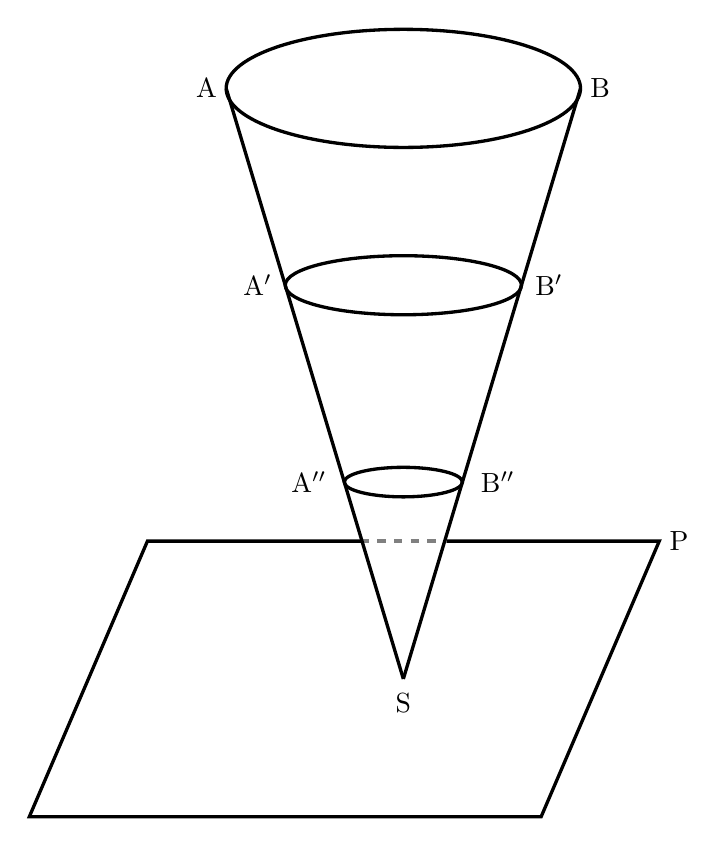
\begin{tikzpicture}	
	%parallelogram
	\draw[very thick] (3.25,1.75)--(-3.25,1.75)--(-4.75,-1.75)--(1.75,-1.75)--cycle;
	\draw[ultra thick,white] (-0.54,1.75)--(0.55,1.75);
	\draw[very thick,dashed,gray] (-0.54,1.75)--(0.55,1.75);
	
	%triangle
	\draw[very thick] (0,0)--(-2.25,7.5);	%leftwards line
	\draw[very thick] (0,0)--( 2.25,7.5);	%rightward line
	
	%ellipses
	\draw[very thick] (0,7.5) ellipse (2.25cm and 0.75cm);
	\draw[very thick] (0,5.0) ellipse (1.5cm and 0.375cm);
	\draw[very thick] (0,2.5) ellipse (0.75cm and 0.1875cm);
	
	%labels
	\node at (0,-0.3)	{S};
	\node at (3.5,1.75) {P};
	\node at (-2.5,7.5) {A};	\node at (-1.85,5)	{A$'$};		\node at (-1.2,2.5) {A$''$};
	\node at ( 2.5,7.5) {B};	\node at ( 1.85,5)	{B$'$};		\node at ( 1.2,2.5) {B$''$};
	\end{tikzpicture}
	%see also O'Sullivan (2013) for some variations on this diagram
	%https://www.simonosullivan.net/articles/bergsonian-production-of-subjectivity.pdf
	
\end{document}